\documentclass[11pt]{article}
\usepackage[english]{babel}
\usepackage{minted}
\usepackage{amsfonts}
\usepackage{amsmath}
\usepackage{amsthm}
\usepackage{graphicx}
\usepackage{subcaption}
\usepackage{booktabs}
\usepackage[left=25mm, top=25mm, bottom=25mm, right=25mm]{geometry}
\usepackage{algorithm}
\usepackage{algpseudocode}
\usepackage[most]{tcolorbox}
\usepackage[colorlinks=true,linkcolor=darkcyan,filecolor=darkcerulean,urlcolor=magenta]{hyperref}

\newtheorem{theorem}{Theorem}[section]
\newtheorem{claim}[theorem]{Claim}
\newtheorem*{question}{Question}

\newtcolorbox{solution}[2][]{breakable,enhanced,adjusted title={#2},colback=codegray,colframe=codegray!50!black}

\linespread{1.0}

\definecolor{codegray}{rgb}{0.98,0.97,0.93}
\definecolor{cottoncandy}{rgb}{1.0, 0.74, 0.85}
\definecolor{darkcerulean}{rgb}{0.03, 0.27, 0.49}
\definecolor{darkcyan}{rgb}{0.0, 0.50, 0.45}

\title{COL718 Assignment 2 Report}
\author{Sayam Sethi (2019CS10399)\\Rishi Sarraf (2019CS10393)}
\date{October 2022}

\begin{document}

\maketitle

\tableofcontents

\pagenumbering{arabic}

\section{Implementation}
We implementated the required functionality for system calls and clflush in the existing Tejas codebase. New classes have been defined wherever necessary. Most of our implementation has used the pre-existing pattern of code by making suitable changes. A few functions have been defined to handle execution of the new instruction types. The structure of implementation is similar for both instruction types:
\begin{enumerate}
    \item New instruction types \texttt{SYSCALL} and \texttt{CLFLUSH} are defined in \texttt{InstructionClass.java}
\begin{figure}
\centering
\begin{minipage}{.5\textwidth}
  \centering
  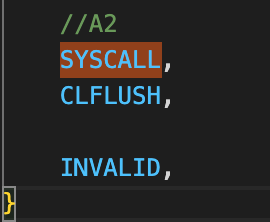
\includegraphics[width=0.6\linewidth]{screenshots/InstructionClass.png}
  \captionof{figure}{\texttt{InstructionClass.java}}
  \label{fig:IC}
\end{minipage}%
\begin{minipage}{.55\textwidth}
  \centering
  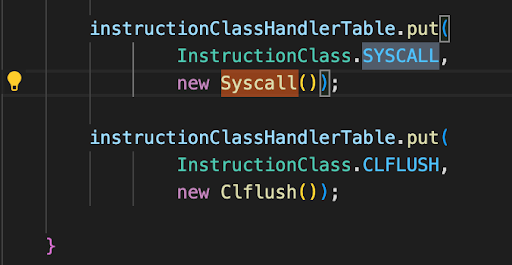
\includegraphics[width=0.8\linewidth]{screenshots/InstructionClassTable2.png}
  \captionof{figure}{\texttt{InstructionClassTable.java}}
  \label{fig:ICT2}
\end{minipage}
\end{figure}
    \item New handler classes \texttt{Syscall} and \texttt{Clflush} are defined in files \texttt{Syscall.java} and \texttt{Clflush.java} for syscall and clflush  (respectively).  
    \item These instruction classes  are added to \texttt{InstructionClassTable} and \texttt{InstructionClassHandlerTable}, these would be needed in the parsing of trace file.
\begin{figure}[H]
\centering
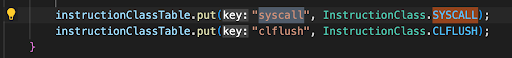
\includegraphics[scale = 0.8]{screenshots/InstructionClassTable1.png}
\caption{\texttt{InstructionClassTable.java}}
\label{fig:ICT1}
\end{figure}
    \item New operation types \texttt{syscall} and \texttt{clflush} are added in \texttt{OperationType.java}
    
    \item These new operation types are mapped to \texttt{FunctionalUnitType.memory} in \texttt{OpTypeToFUTypeMapping.java} as they are memory based operations.
\begin{figure}
\centering
\begin{minipage}{.5\textwidth}
  \centering
  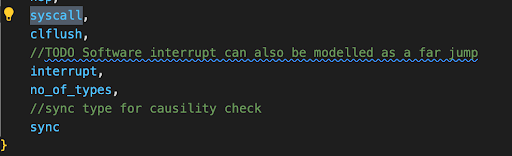
\includegraphics[width=0.9\linewidth]{screenshots/OperationType.png}
  \captionof{figure}{\texttt{OperationType.java}}
  \label{fig:IC}
\end{minipage}%
\begin{minipage}{.55\textwidth}
  \centering
  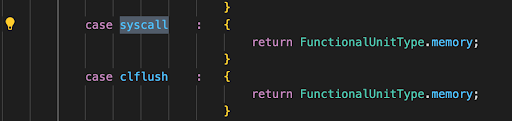
\includegraphics[width=1\linewidth]{screenshots/OpTypeToFUTypeMapping.png}
  \captionof{figure}{\texttt{OpTypeToFUTypeMapping.java}}
  \label{fig:ICT2}
\end{minipage}
\end{figure}    
    \item \textbf{Handling in IW} These instruction are issued in \texttt{issueMemoryInstruction()} in the file \texttt{IWEntry.java}
    \item \textbf{Commit} Execution occurs similar to \texttt{store} instructions. They are executed at commit time, i.e., when they are at the top of ROB. Hence, in \texttt{performCommits()} in \texttt{ReorderBuffer.java}, they are handled in if blocks with condition evaluating \texttt{firstOpType == OperationType.syscall}
\begin{figure}[H]
\centering
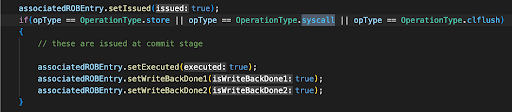
\includegraphics[scale = 0.8]{screenshots/IWWrite1.png}
\caption{\texttt{IWWrite.java}}
\label{fig:IWW1}
\end{figure}
    \item New request types \texttt{Tlb\_Flush} and \texttt{Cache\_Line\_Flush} are added in \texttt{RequestType.java} for creating events corresponding to execution of these instructions.
\begin{figure}[H]
\centering
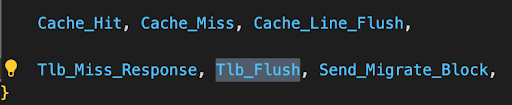
\includegraphics[scale = 0.6]{screenshots/RequestType.png}
\caption{\texttt{RequestType.java}}
\label{fig:RT}
\end{figure}
    \item Visa Handlers  \texttt{Syscall} and \texttt{Clflush} are defined in files \texttt{Syscall.java} and \texttt{Clflush.java} (in directory visaHandler) for syscall and clflush  (respectively).
    \item These handlers are instantiated in \texttt{VisaHandler.java}.
    \item These are used to parse the address arguments and help with creation of the tail of instruction packets.
\begin{figure}
\centering
\begin{minipage}{.5\textwidth}
  \centering
  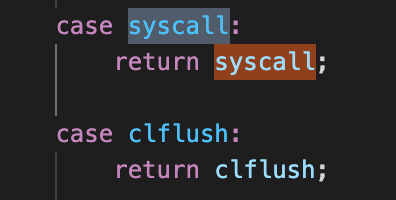
\includegraphics[width=0.55\linewidth]{screenshots/VisaHandler1.png}
  \captionof{figure}{\texttt{VisaHandler.java}}
  \label{fig:VH1}
\end{minipage}%
\begin{minipage}{.55\textwidth}
  \centering
  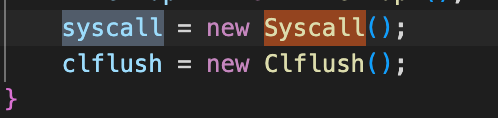
\includegraphics[width=1\linewidth]{screenshots/VisaHandler2.png}
  \captionof{figure}{\texttt{VisaHandler.java}}
  \label{fig:VH2}
\end{minipage}
\end{figure}   
\end{enumerate}

The above flow explains where in code their execution function can be called. In Tejas, execute steps are event-driven. We thus need to create `events' with appropriate arguments in order to call the desired execute functions.
\subsection{System calls (syscall)}
An event based mechanism is used to handle the execution of \texttt{syscall}. An request type called \texttt{Tlb\_Flush} has been defined and and event with this request type is added to the event queue in \texttt{performCommits()} function defined in \texttt{ReorderBuffer.java}. The event handler of TLB is responsible for calling the \texttt{flush()} function defined in \texttt{TLB.java}. The flush function just instantiates a new hashtable thus `flushing' the TLB effectively.
\begin{figure}[H]
\centering
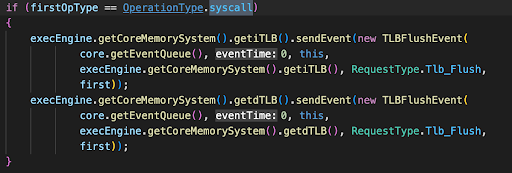
\includegraphics[scale = 0.6]{screenshots/ReorderBufferSyscall.png}
\caption{\texttt{ReorderBuffer.java}}
\label{fig:RBSys}
\end{figure}
\begin{figure}[H]
\centering
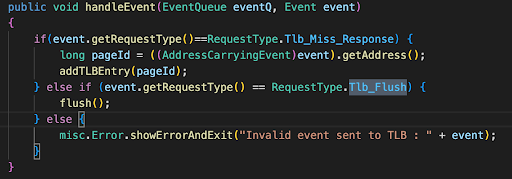
\includegraphics[scale = 0.6]{screenshots/TLBHandleEvent.png}
\caption{\texttt{TLB.java}}
\label{fig:TLBHE}
\end{figure}
\begin{figure}[H]
\centering
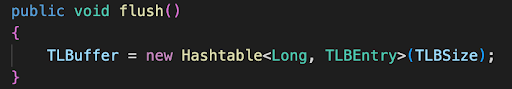
\includegraphics[scale = 0.6]{screenshots/TLBFlush.png}
\caption{\texttt{TLB.java}}
\label{fig:TLBFlush}
\end{figure}
\subsection{Clflush}
A similar mechanism is used to handle the execution of \texttt{clflush}. An request type called \texttt{Cachle\_Line\_Flush} has been defined and and event with this request type is added to the event queue in \texttt{performCommits()} function defined in \texttt{ReorderBuffer.java}. The event handler of Cache is responsible for calling the \texttt{handleCacheLineFlush()} function defined in \texttt{Cache.java}. This function recursively sends events invalidating all cache levels and eventually writes to memory.
\begin{figure}[H]
\centering
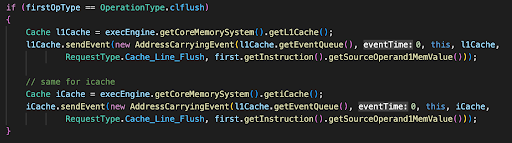
\includegraphics[scale = 0.6]{screenshots/ReorderBufferClflush.png}
\caption{\texttt{ReorderBuffer.java}}
\label{fig:RBSys}
\end{figure}
\begin{figure}[H]
\centering
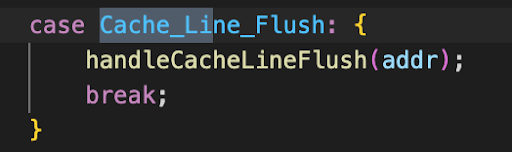
\includegraphics[scale = 0.4]{screenshots/CacheHandleEvent.png}
\caption{\texttt{Cache.java}}
\label{fig:TLBHE}
\end{figure}
\begin{figure}[H]
\centering
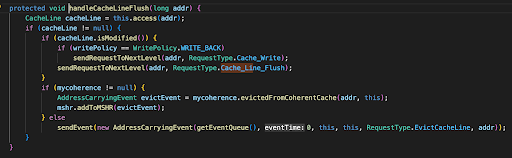
\includegraphics[scale = 0.6]{screenshots/CacheFlush.png}
\caption{\texttt{Cache.java}}
\label{fig:TLBFlush}
\end{figure}

\newpage

\section{Statistics}
The following table summarises the simulation statistics for different scenerios, i.e., with and without flushing TLB and Cachelines.
\begin{table}[h]
    \centering
    \makebox[\textwidth][c]{
    \begin{tabular}{|c|c|c|c|c|}
        \toprule
         Quantity & noflush & tlbflush & clflush & tlbclflush\\
        \hline
          IPC(micro-ops) & 0.2574  & 0.2522  & 0.2574  & 0.2522 \\
        %  \hline
          iTLB hits & 78860 & 78514 & 78860 & 78514 \\
          iTLB misses & 474 & 815 & 474 & 815 \\
          dTLB hits & 29456 & 29225 & 29455 & 29224 \\
          dTLB misses & 132 & 361 & 132 & 361 \\
          L1 hits & 25447 & 25466  & 25444 & 25463\\
          L1 misses & 1439 & 1433 & 1440 & 1434\\
          L2 hits &6799  & 6808 & 6799 & 6808\\
          L2 misses &1541 & 1540 & 1541 & 1540\\
          L3 hits & 432 & 430 & 432 & 430 \\
          L3 misses &1314 & 1314 & 1314 & 1314 \\
          I1 hits &74342 & 74340 & 74342 & 74340\\
          I1 misses &4986  & 4979 & 4986 & 4979 \\
          Directory Access EvictionFromCoherentCache & 41 & 41 & 42 & 42\\
          Coherence energy & 42277.33 &  43149.6216 & 42278.01 & 43150.3008	\\
          
        \bottomrule
    \end{tabular}
    }
    \caption{Simulation Statistics Comparison.}\label{tab:sim_stats}
\end{table}
\subsection{Simulation observations:}
\begin{enumerate}
    \item TLB flush decreases the IPC, whereas CL Flush doesn't. This is becuase TLB misses increases significantly (almost 2 fold) and in our simulation. CL FLush doesn't significantly change cache hit/miss rates.
    \item TLB flush increases the iTLB and dTLB misses (thus decreasing the hits). This is an expected behaviour, flushing the TLB will lead to TLB misses. CL Flush has no impact on TLB stats.
    \item CL Flush decreases L1 hits and increases L1 misses. It does not, however, change the stats at other levels.
    % \item TLB Flush increases cache hits. \textcolor{red}{Why?}
    \item CL Flush increases directory accesses due to eviction from coherent caches.
    \item CL Flush and TLB Flush increase coherence energy.
    \item TLB Flush and CL Flush seem to independently change coherence energy and the effect of (TLB+CL) Flush is the sum of individual flush effects.
\end{enumerate}

\end{document}